%% WalkMode — report draft (ACM sigconf).
%% Compile on Overleaf (acmart is built in) or locally with: latexmk -pdf walkmode.tex
%% Numbers, tables and figures in the Results section are generated by analysis/analyze.py into generated/.
%% Lines marked \todo{...} need your input. Search for "TODO" before submitting.

\documentclass[sigconf,nonacm]{acmart}

\usepackage{booktabs}
\usepackage{tikz}
\usetikzlibrary{arrows.meta,positioning}
\usepackage{xcolor}

\newcommand{\todo}[1]{\textcolor{red}{[TODO: #1]}}
\newcommand{\WM}{\textsc{WalkMode}}

% Generated by analysis/analyze.py
% Generated by analysis/analyze.py — do not edit by hand.
\newcommand{\DataSource}{SYNTHETIC}
\newcommand{\IsSynthetic}{1}
\newcommand{\NP}{12}
\newcommand{\StatTimeIface}{$F(1,11)=3.98$, $p=.071$, $\eta_p^2=0.27$}
\newcommand{\StatTimeMob}{$F(1,11)=228.80$, $p<.001$, $\eta_p^2=0.95$}
\newcommand{\StatTimeInter}{$F(1,11)=5.07$, $p=.046$, $\eta_p^2=0.32$}
\newcommand{\CmpTimeWalk}{$t(11)=-3.32$, $p_{Holm}=.014$, $d_z=-0.96$}
\newcommand{\CmpTimeStand}{$t(11)=-0.06$, $p_{Holm}=.951$, $d_z=-0.02$}
\newcommand{\MeanTimeStdStand}{2.20}
\newcommand{\MeanTimeWmStand}{2.19}
\newcommand{\MeanTimeStdWalk}{2.73}
\newcommand{\MeanTimeWmWalk}{2.58}
\newcommand{\StatErrorsIface}{$F(1,11)=11.13$, $p=.007$, $\eta_p^2=0.50$}
\newcommand{\StatErrorsMob}{$F(1,11)=20.12$, $p<.001$, $\eta_p^2=0.65$}
\newcommand{\StatErrorsInter}{$F(1,11)=11.00$, $p=.007$, $\eta_p^2=0.50$}
\newcommand{\CmpErrorsWalk}{$W=1$, $p_{Holm}=.031$, $r=-0.84$}
\newcommand{\CmpErrorsStand}{$W=0$, $p_{Holm}=1.000$, $r=-1.00$}
\newcommand{\MeanErrorsStdStand}{0.00}
\newcommand{\MeanErrorsWmStand}{0.00}
\newcommand{\MeanErrorsStdWalk}{0.11}
\newcommand{\MeanErrorsWmWalk}{0.01}
\newcommand{\StatMissesIface}{$F(1,11)=3.26$, $p=.098$, $\eta_p^2=0.23$}
\newcommand{\StatMissesMob}{$F(1,11)=36.14$, $p<.001$, $\eta_p^2=0.77$}
\newcommand{\StatMissesInter}{$F(1,11)=3.94$, $p=.073$, $\eta_p^2=0.26$}
\newcommand{\CmpMissesWalk}{$W=16.5$, $p_{Holm}=.156$, $r=-0.51$}
\newcommand{\CmpMissesStand}{$W=3$, $p_{Holm}=.375$, $r=0.54$}
\newcommand{\MeanMissesStdStand}{0.02}
\newcommand{\MeanMissesWmStand}{0.04}
\newcommand{\MeanMissesStdWalk}{0.16}
\newcommand{\MeanMissesWmWalk}{0.08}
\newcommand{\StatTlxIface}{$F(1,11)=16.93$, $p=.002$, $\eta_p^2=0.61$}
\newcommand{\StatTlxMob}{$F(1,11)=705.99$, $p<.001$, $\eta_p^2=0.98$}
\newcommand{\StatTlxInter}{$F(1,11)=6.42$, $p=.028$, $\eta_p^2=0.37$}
\newcommand{\CmpTlxWalk}{$W=5.5$, $p_{Holm}=.011$, $r=-0.76$}
\newcommand{\CmpTlxStand}{$W=18$, $p_{Holm}=.373$, $r=-0.31$}
\newcommand{\MeanTlxStdStand}{18.00}
\newcommand{\MeanTlxWmStand}{17.29}
\newcommand{\MeanTlxStdWalk}{36.46}
\newcommand{\MeanTlxWmWalk}{30.70}
\newcommand{\TimeRatioWalk}{5}
\newcommand{\TostStand}{ratio $=1.00$, 90\% CI [0.96, 1.03], $p<.001$}
\newcommand{\PrefStanding}{5 WalkMode, 1 Standard, 6 no preference (binomial $p=.219$)}
\newcommand{\PrefWalking}{10 WalkMode, 0 Standard, 2 no preference (binomial $p=.002$)}
\newcommand{\PrefOverall}{6 WalkMode, 3 Standard, 3 no preference (binomial $p=.508$)}
\newcommand{\DetWalkPct}{96}
\newcommand{\DetLatency}{2.8}
\newcommand{\DetFalsePos}{1 of 24}

% Generated by analysis/analyze.py — do not edit by hand.
\newcommand{\DescriptivesTable}{%
\begin{tabular}{@{}lrrrr@{}}
\toprule
Measure & Standard\,/\,Standing & WalkMode\,/\,Standing & Standard\,/\,Walking & WalkMode\,/\,Walking \\
\midrule
Completion time (s) & 2.20 (0.53) & 2.19 (0.43) & 2.73 (0.69) & 2.58 (0.58) \\
Selection errors / trial & 0.00 (0.01) & 0.00 (0.00) & 0.11 (0.10) & 0.01 (0.02) \\
Missed taps / trial & 0.02 (0.04) & 0.04 (0.06) & 0.16 (0.13) & 0.08 (0.07) \\
NASA-TLX (0-100) & 18.00 (8.15) & 17.29 (6.97) & 36.46 (7.99) & 30.70 (9.39) \\
\bottomrule
\end{tabular}}

\newcommand{\AnovaTable}{%
\begin{tabular}{@{}lccc@{}}
\toprule
Measure & Interface & Mobility & Interface $\times$ Mobility \\
\midrule
Completion time (s) & 3.98, $p=.071$, 0.27 & 228.80, $p<.001$, 0.95 & 5.07, $p=.046$, 0.32 \\
Selection errors / trial & 11.13, $p=.007$, 0.50 & 20.12, $p<.001$, 0.65 & 11.00, $p=.007$, 0.50 \\
Missed taps / trial & 3.26, $p=.098$, 0.23 & 36.14, $p<.001$, 0.77 & 3.94, $p=.073$, 0.26 \\
NASA-TLX (0-100) & 16.93, $p=.002$, 0.61 & 705.99, $p<.001$, 0.98 & 6.42, $p=.028$, 0.37 \\
\bottomrule
\end{tabular}}

\newcommand{\PlannedTable}{%
\begin{tabular}{@{}lll@{}}
\toprule
Measure & Walking: WalkMode vs Standard & Standing: WalkMode vs Standard \\
\midrule
Completion time (s) & $t(11)=-3.32$, $p_{Holm}=.014$, $d_z=-0.96$ & $t(11)=-0.06$, $p_{Holm}=.951$, $d_z=-0.02$ \\
Selection errors / trial & $W=1$, $p_{Holm}=.031$, $r=-0.84$ & $W=0$, $p_{Holm}=1.000$, $r=-1.00$ \\
Missed taps / trial & $W=16.5$, $p_{Holm}=.156$, $r=-0.51$ & $W=3$, $p_{Holm}=.375$, $r=0.54$ \\
NASA-TLX (0-100) & $W=5.5$, $p_{Holm}=.011$, $r=-0.76$ & $W=18$, $p_{Holm}=.373$, $r=-0.31$ \\
\bottomrule
\end{tabular}}

\newcommand{\SyntheticBanner}{%
  \ifnum\IsSynthetic=1
  \par\noindent\fcolorbox{red}{red!8}{\parbox{\dimexpr\linewidth-2\fboxsep-2\fboxrule}{\small\textbf{Placeholder results.}
  All numbers, tables and figures in this section were produced from \emph{synthetic} sessions
  (\texttt{analysis/make\_synthetic.py}) to test the analysis pipeline. Replace them by running
  \texttt{analysis/analyze.py} on the real study data, then rewrite the prose.}}\par\medskip
  \fi}

\begin{document}

\title{WalkMode: Movement-Aware Touch Targets for Mobile Interaction While Walking}

\author{Anh Nguyen}
\affiliation{%
  \institution{Stony Brook University}
  \city{Stony Brook}
  \state{New York}
  \country{USA}}
\email{anh.nguyen.3@stonybrook.edu}

\begin{abstract}
Mobile devices are frequently used while walking, yet most mobile interfaces keep the same layout regardless of whether the user is stationary or moving. Walking reduces touch accuracy, increases interaction time, and makes small interface elements difficult to select. We present \WM{}, a movement-aware mobile web interface that uses the smartphone's accelerometer to detect walking and automatically enlarges touch targets and the spacing between them; the standard layout is restored when the user stops. A lightweight detector combines the variability of body acceleration with step rhythm and hysteresis, and a touch-aware switching policy prevents the layout from changing under the user's finger. We evaluated \WM{} in a 2$\times$2 within-subjects study (Interface: Standard, \WM{} $\times$ Mobility: Standing, Walking) with \NP{} participants performing app-selection, list-selection and settings-navigation tasks, measuring task completion time, selection errors, missed taps, perceived workload (NASA-TLX) and preference. \todo{One or two sentences summarising the main findings once the real data are analysed.}
\end{abstract}

\begin{CCSXML}
<ccs2012>
<concept><concept_id>10003120.10003138.10011767</concept_id>
<concept_desc>Human-centered computing~Empirical studies in ubiquitous and mobile computing</concept_desc>
<concept_significance>500</concept_significance></concept>
<concept><concept_id>10003120.10003121.10003125.10011752</concept_id>
<concept_desc>Human-centered computing~Touch screens</concept_desc>
<concept_significance>300</concept_significance></concept>
</ccs2012>
\end{CCSXML}
\ccsdesc[500]{Human-centered computing~Empirical studies in ubiquitous and mobile computing}
\ccsdesc[300]{Human-centered computing~Touch screens}

\keywords{situational impairments, walking user interfaces, adaptive interfaces, target size, mobile interaction, context awareness}

\maketitle

%% =====================================================================
\section{Introduction}

People routinely read messages, pick songs, look up directions and change settings on their phones while walking. Walking is a \emph{situational impairment}~\cite{sears2003fade}: the rhythmic motion of the body moves both the phone and the finger, divides attention between the screen and the environment, and measurably degrades touch performance. Studies of walking interaction report slower selection, more errors and lower reading performance than when standing~\cite{lin2007tap,kane2008walking,schildbach2010walking,bergstrom2011speed}, and the decline grows with walking speed~\cite{bergstrom2011speed,mizobuchi2005walking}.

Despite this, mainstream mobile interfaces present one layout for every context. Their targets are sized for a user who is standing or sitting still, which is exactly when users need help the least. Prior work has shown that larger targets reduce the cost of walking~\cite{kane2008walking,schildbach2010walking}, but permanently enlarging everything wastes screen space and requires more scrolling when the user is stationary.

This project asks whether a \emph{simple, automatic} adaptation is enough: detect walking with the phone's own accelerometer, enlarge touch targets and spacing only while the user walks, and restore the standard layout when they stop. Our contributions are:
\begin{itemize}
  \item \WM{}, a mobile web interface that adapts target size and spacing to walking. It uses an interpretable walking detector (motion variability, step cadence, rhythm regularity and hysteresis) and a \emph{touch-idle} switching policy that never moves targets under the user's finger.
  \item An open study apparatus that runs in a phone browser: counterbalanced conditions, three common selection and navigation tasks, tap-level logging, NASA-TLX and preference questionnaires, and data export.
  \item A controlled 2$\times$2 within-subjects evaluation comparing the Standard and \WM{} interfaces while standing and walking. \todo{Summarise the headline result.}
\end{itemize}

%% =====================================================================
\section{Related Work}

\subsection{Walking as a situational impairment}
Sears et al.~\cite{sears2003fade} framed environmental and contextual factors such as motion as \emph{situationally-induced impairments}, which call for the same design attention as permanent disabilities. Ability-based design~\cite{wobbrock2011ability} likewise argues that systems should adapt to what users can do in the moment. Empirical studies consistently find that walking degrades touch input. Lin et al.~\cite{lin2007tap} measured stylus tapping on a treadmill and found that walking lowered accuracy and increased workload, especially for small targets. Kane et al.~\cite{kane2008walking} evaluated \emph{walking user interfaces} in public spaces and reported that larger targets improved performance while walking. Schildbach and Rukzio~\cite{schildbach2010walking} showed that walking reduced both target-selection and reading performance, and that larger targets compensated only partly. Bergstrom-Lehtovirta et al.~\cite{bergstrom2011speed} found that accuracy falls as walking speed increases, and Crossan et al.~\cite{crossan2005gait} showed that tap accuracy varies with gait phase. Later work modelled the systematic offsets of touches made while walking~\cite{music2016nomadic} and the effect of carrying objects~\cite{ng2014encumbrance}.

\subsection{Target size on touchscreens}
For one-handed thumb use, Parhi et al.~\cite{parhi2006target} recommended targets of at least about 9.2\,mm for discrete tasks, larger than many interface elements in practice. A fixed layout therefore faces a trade-off. Targets large enough for walking waste space when stationary, while compact layouts are hard to hit on the move. \WM{} resolves the trade-off over time instead of in space: it enlarges targets only when the context requires it.

\subsection{Sensing context to adapt interaction}
Accelerometers reliably distinguish walking from standing~\cite{kwapisz2011activity}. WalkType~\cite{goel2012walktype} used accelerometer data to correct text entry while walking by adjusting key classification under the hood. \WM{} takes a complementary, \emph{visible} approach: it changes the layout itself. Visible adaptation carries known risks. Adaptive interfaces can disorient users when items move unpredictably~\cite{findlater2004menus,gajos2006adaptive}. \WM{}'s design therefore limits adaptation to geometry (sizes and spacing, not order), signals each change, and defers it until the user is not touching the screen.

%% =====================================================================
\section{WalkMode}

\begin{figure}[t]
\centering
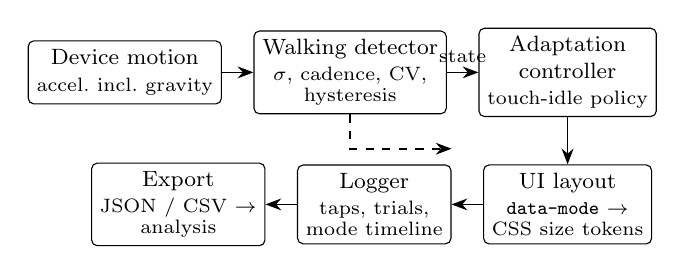
\begin{tikzpicture}[
  box/.style={draw, rounded corners=2pt, align=center, font=\footnotesize, minimum height=8mm, inner sep=3pt, fill=white},
  arr/.style={-{Stealth[length=2mm]}, semithick}]
  \node[box] (sens) {Device motion\\\scriptsize accel.\ incl.\ gravity};
  \node[box, right=4mm of sens] (det) {Walking detector\\\scriptsize $\sigma$, cadence, CV,\\[-2pt]\scriptsize hysteresis};
  \node[box, right=4mm of det] (adapt) {Adaptation\\controller\\\scriptsize touch-idle policy};
  \node[box, below=6mm of adapt] (ui) {UI layout\\\scriptsize \texttt{data-mode} $\rightarrow$\\[-2pt]\scriptsize CSS size tokens};
  \node[box, left=4mm of ui] (log) {Logger\\\scriptsize taps, trials,\\[-2pt]\scriptsize mode timeline};
  \node[box, left=4mm of log] (exp) {Export\\\scriptsize JSON / CSV $\rightarrow$\\[-2pt]\scriptsize analysis};
  \draw[arr] (sens) -- (det);
  \draw[arr] (det) -- node[above, font=\scriptsize]{state} (adapt);
  \draw[arr] (adapt) -- (ui);
  \draw[arr] (ui) -- (log);
  \draw[arr] (log) -- (exp);
  \draw[arr, dashed] (det.south) |- ([yshift=2mm]log.north east) ;
\end{tikzpicture}
\caption{\WM{} architecture. The detector's state drives the adaptation controller, which switches the UI between the standard and walking size tokens. Every state change, mode change and tap is logged.}
\label{fig:arch}
\end{figure}

\WM{} is a static mobile web application written in HTML, CSS and JavaScript, with no build step and no server. It runs in any modern phone browser over HTTPS, a requirement for motion-sensor access. Figure~\ref{fig:arch} shows the architecture.

\subsection{Walking detection}
\label{sec:detector}
The detector uses the \texttt{devicemotion} event's \emph{acceleration including gravity}, because it is the most widely available stream. Each sample $\mathbf{a}_t$ is reduced to its magnitude $m_t=\lVert\mathbf{a}_t\rVert$, which does not depend on how the phone is held. Gravity is tracked with an exponential moving average $g_t = g_{t-1} + \alpha_t(m_t-g_{t-1})$, where $\alpha_t = 1-e^{-\Delta t/\tau_g}$ and $\tau_g=1$\,s. The residual $m_t-g_t$ is smoothed lightly ($\tau=40$\,ms) to give the dynamic acceleration $d_t$. Every 100\,ms the detector computes three features over the last $W=2.5$\,s of $d$:
\begin{itemize}
  \item the standard deviation $\sigma$ (motion energy);
  \item the step cadence $f = 1/\overline{\Delta t}$, from peaks above $\mu + 0.6\sigma$ spaced at least 0.3\,s apart;
  \item the coefficient of variation (CV) of the inter-peak intervals (rhythm regularity).
\end{itemize}
A window is \emph{walking-like} when $\sigma \ge \theta_{in}$, $f \in [1.2, 3.0]$\,Hz and CV $\le 0.45$. The cadence and rhythm conditions reject the irregular jolts that tapping produces while the user stands. A window is \emph{still-like} when $\sigma < \theta_{out}$ or no rhythmic stepping is present. The state switches to \emph{walking} after 1.2\,s of consecutive walking-like windows, and back to \emph{stationary} after 2.5\,s of still-like windows. This asymmetric hysteresis keeps a brief pause, such as waiting at a door, from flipping the layout. In simulation the detector switched on about 2.6\,s after walking began and off about 4\,s after it stopped. It ignored tap jolts and 1.5\,s pauses (unit tests in \texttt{tests/detector.test.mjs}).

The default thresholds are $\theta_{in}=0.6$ and $\theta_{out}=0.35$\,m/s$^2$. Because gait and grip vary, an optional 25-second calibration records the participant's typical $\sigma$ while standing and tapping ($\sigma_s$) and while walking ($\sigma_w$), and sets $\theta_{in}=\sigma_s+0.4(\sigma_w-\sigma_s)$ and $\theta_{out}=\sigma_s+0.2(\sigma_w-\sigma_s)$.

\subsection{Adaptation}
All interface dimensions are CSS custom properties generated from one configuration file, and a single attribute on the root element (\texttt{data-mode}) selects the standard or the walking set (Table~\ref{tab:sizes}). In walking mode, target sizes grow by about 60\%, gaps between targets roughly triple, text grows by 3\,px, and the app grid drops from five columns to four so that the larger icons still fit without scrolling. Only geometry changes. The order of items and the navigation structure stay the same, which avoids the disorientation that comes with adaptive reordering~\cite{findlater2004menus}. A small ``Walking mode'' indicator in the header makes the state visible.

\begin{table}[t]
\caption{Interface dimensions (CSS px; 1\,px $\approx$ 0.16\,mm on typical phones).}
\label{tab:sizes}
\small
\begin{tabular}{@{}lrr@{}}
\toprule
Element & Standard & Walking \\
\midrule
App icon (grid) & 40 ($\approx$6.3\,mm) & 64 ($\approx$10.2\,mm) \\
Gap between targets & 6 & 16 \\
Grid columns & 5 & 4 \\
List / menu row height & 44 & 64 \\
Back button & 36 & 56 \\
Toggle switch & 40$\times$24 & 60$\times$36 \\
Body / prompt text & 15 / 17 & 18 / 21 \\
\bottomrule
\end{tabular}
\end{table}

\paragraph{Touch-idle switching.} Changing the layout while a finger is on its way to a target would turn the adaptation itself into a source of errors. \WM{} therefore defers a pending change while any pointer is down and until 700\,ms after the last touch ends, then applies it with a 200\,ms transition. In the scrolling contact list, the row at the top of the viewport keeps its position across the change. The deferral time and the alternative policies (\emph{immediate}, \emph{between trials}) are configurable.

\subsection{Implementation and logging}
The app runs as a hash-routed single-page application, and the Screen Wake Lock API keeps the display on during sessions. Taps are recognised from pointer events (movement $\le$ 15\,px, duration $\le$ 800\,ms), and the hit target is resolved where the finger \emph{lands}. Each tap is classified as a \emph{hit} (the element the current step requires), a \emph{selection error} (a different interactive element) or a \emph{miss} (no interactive element: a gap, a label or the background). Taps that stop a momentum scroll and taps on app chrome are logged separately and excluded. For every tap the logger stores coordinates, the offset from the intended target's centre and its size, the current layout mode and the detector state. It also keeps per-trial timing, a 1\,Hz motion summary and the full timeline of detector and layout changes. Sessions autosave to the browser's local storage after every trial and are exported as JSON and CSV through the share sheet or a download.

%% =====================================================================
\section{User Study}

\subsection{Hypotheses}
\begin{description}
  \item[H1] While walking, \WM{} reduces selection errors and missed taps compared with the Standard interface.
  \item[H2] While walking, \WM{} reduces task completion time compared with the Standard interface.
  \item[H3] While standing, \WM{} performs equivalently to the Standard interface, because the adaptation stays inactive.
  \item[H4] While walking, \WM{} lowers perceived workload (NASA-TLX).
  \item[H5] Participants prefer \WM{} for use while walking.
\end{description}

\subsection{Participants}
\todo{N = \NP{}; recruitment; age range; gender; handedness; phone OS and daily use; how often they use a phone while walking (all collected by the app's setup form); compensation, if any.} Participants held the phone in their dominant hand and interacted with that hand's thumb.

\subsection{Apparatus}
\todo{Phone model, OS and browser version, screen size; whether participants used one study phone or their own (record what you did).} The app was served over HTTPS from GitHub Pages and added to the home screen to hide browser chrome. Walking took place on \todo{describe route: an indoor corridor loop of about N\,m, free of obstacles and stairs}. The experimenter walked behind the participant for safety.

\subsection{Tasks}
Each block contained three tasks, always in the same order. Stimulus positions were re-randomised on every trial with a seeded generator, so participants could not memorise locations.
\begin{description}
  \item[App launcher (10 trials).] A 20-icon grid. The prompt names one app (e.g., ``Open \emph{Camera}''), and the participant taps it.
  \item[Contacts (6 trials).] An alphabetised list of 40 names. The participant scrolls to the named contact and taps it, and the target usually lies below the fold.
  \item[Settings (5 trials).] A two-level settings menu (eight categories with six toggle switches each). The participant opens the named category and switches the named setting \textsc{on} or \textsc{off}, using the back button to recover from a wrong page.
\end{description}
A trial ended with the correct selection or after a timeout (15, 20 and 25\,s for the three tasks). Wrong selections produced brief visual feedback, plus vibration where supported.

\subsection{Design}
The study used a 2 (Interface: Standard, \WM{}) $\times$ 2 (Mobility: Standing, Walking) within-subjects design. The four conditions were counterbalanced with a balanced Latin square~\cite{williams1949latin}, so each condition appears once in each position and each condition follows every other exactly once across four orders. The detector ran in every condition, but in the Standard interface it only logged and never changed the layout. Each participant completed 4 blocks $\times$ 21 trials = 84 measured trials.

\subsection{Procedure}
After consent and the demographic questions, participants optionally completed the detector calibration (Section~\ref{sec:detector}). Next came a practice round with every task in both layouts. Each block began with an instruction screen: for walking blocks, participants started walking the route before tapping \emph{Start}. A 3-second countdown let the detector settle. After each block, participants completed the raw NASA-TLX~\cite{hart1988tlx,hart2006tlx}. A final questionnaire asked which interface they preferred while standing, while walking and overall. It also had five 7-point Likert items (the change was noticeable, disruptive and helpful; detection was accurate; they would use \WM{}) and open comments. Sessions lasted about \todo{N} minutes.

\subsection{Measures and analysis}
\emph{Completion time} is the geometric mean duration of successful trials per participant and condition, analysed on a log scale. \emph{Selection errors} and \emph{missed taps} are counts per trial. \emph{Workload} is the raw TLX, the unweighted mean of six 0--100 scales. Each measure was analysed with a 2$\times$2 repeated-measures ANOVA. With two levels per factor every effect has one degree of freedom, so sphericity does not apply. For the planned comparisons (\WM{} vs.\ Standard within each mobility level), we used paired $t$-tests on log time and Wilcoxon signed-rank tests for the count and TLX measures. Both were Holm-corrected within each measure~\cite{holm1979}. H3 was tested with a two one-sided tests (TOST) equivalence procedure on log time, using $\pm$10\% bounds~\cite{lakens2017tost}. Error bars show within-subject 95\% confidence intervals~\cite{morey2008ci}. Preferences were tested with binomial tests that excluded ``no preference''. We also report how the detector behaved: the share of each block it labelled as walking, its onset latency and the number of layout switches.

%% =====================================================================
\section{Results}
\SyntheticBanner

\todo{Report excluded participants and blocks, timeouts and any restarted blocks.} Table~\ref{tab:desc} gives per-condition means, Table~\ref{tab:anova} the ANOVA results and Table~\ref{tab:planned} the planned comparisons. Figure~\ref{fig:main} shows the four main measures.

\begin{table*}[t]
\caption{Means (SD) per condition (\DataSource; $N=\NP$). Completion time is the geometric mean of successful trials, in seconds.}
\label{tab:desc}
\small
\DescriptivesTable
\end{table*}

\begin{figure*}[t]
\centering
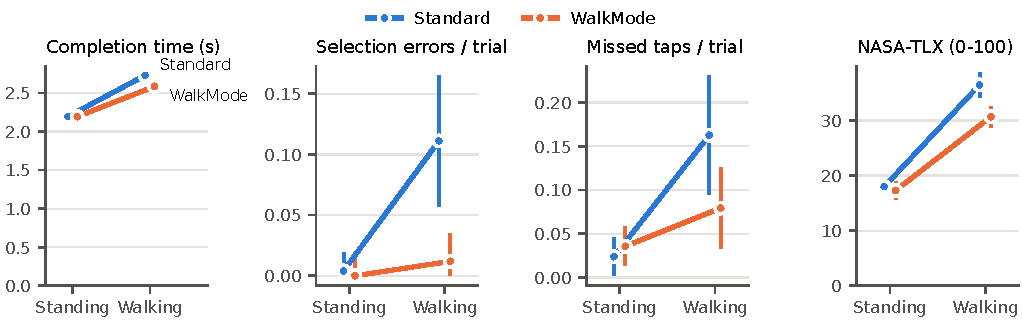
\includegraphics[width=\textwidth]{generated/fig_main.pdf}
\caption{Main measures by interface and mobility (\DataSource). Error bars: within-subject 95\% CIs.}
\label{fig:main}
\end{figure*}

\begin{table*}[t]
\caption{2$\times$2 repeated-measures ANOVA: $F(1,\NP-1)$, $p$, $\eta_p^2$ (\DataSource).}
\label{tab:anova}
\small
\AnovaTable
\end{table*}

\begin{table*}[t]
\caption{Planned comparisons, \WM{} vs.\ Standard (Holm-corrected within each measure; \DataSource).}
\label{tab:planned}
\small
\PlannedTable
\end{table*}

\subsection{Walking detection}
Across walking blocks, the detector labelled about \DetWalkPct\% of block time as walking. Its median onset was \DetLatency\,s after the block started. During standing blocks it reported walking at least once in \DetFalsePos{} blocks. \todo{Interpret: was the adaptation active when it should have been? Were there spurious switches while standing?}

\subsection{Selection errors and missed taps (H1)}
Selection errors: interface \StatErrorsIface; mobility \StatErrorsMob; interaction \StatErrorsInter. While walking, \WM{} vs.\ Standard: \CmpErrorsWalk{} (means \MeanErrorsWmWalk{} vs.\ \MeanErrorsStdWalk{} errors per trial). Missed taps: interaction \StatMissesInter; walking comparison \CmpMissesWalk{} (\MeanMissesWmWalk{} vs.\ \MeanMissesStdWalk{} per trial). Figure~\ref{fig:taps} shows tap offsets relative to target size in the app-launcher task. \todo{State whether H1 is supported, and for which measure.}

\begin{figure}[t]
\centering
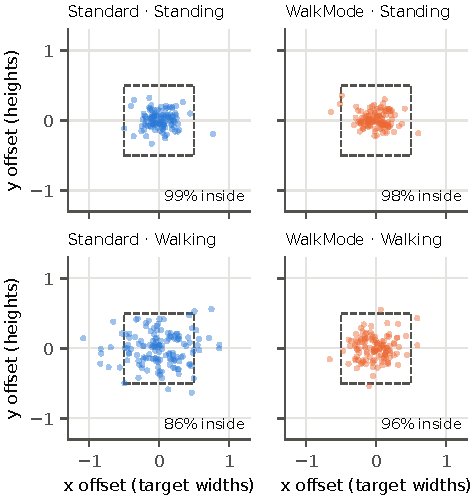
\includegraphics[width=\columnwidth]{generated/fig_taps.pdf}
\caption{Tap offsets in the app-launcher task, normalised by the size of the intended target (dashed box = target), with the percentage of taps landing inside (\DataSource).}
\label{fig:taps}
\end{figure}

\subsection{Completion time (H2, H3)}
Interface \StatTimeIface; mobility \StatTimeMob; interaction \StatTimeInter. While walking, \WM{} vs.\ Standard: \CmpTimeWalk{} (geometric means \MeanTimeWmWalk\,s vs.\ \MeanTimeStdWalk\,s). While standing: \CmpTimeStand{} (\MeanTimeWmStand\,s vs.\ \MeanTimeStdStand\,s); equivalence test: \TostStand. \todo{State whether H2 and H3 are supported. Note any per-task differences (Figure~\ref{fig:tasks}); for example, the larger walking-mode rows need more scrolling in the contacts task.}

\begin{figure*}[t]
\centering
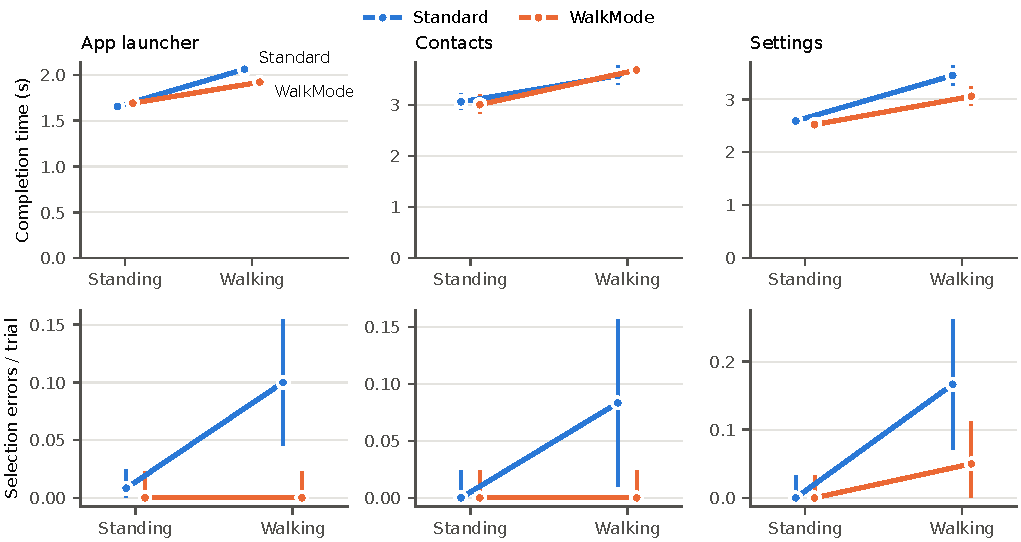
\includegraphics[width=0.85\textwidth]{generated/fig_tasks.pdf}
\caption{Completion time and selection errors per task (\DataSource). Error bars: within-subject 95\% CIs.}
\label{fig:tasks}
\end{figure*}

\subsection{Workload (H4)}
Raw TLX: interface \StatTlxIface; mobility \StatTlxMob; interaction \StatTlxInter. While walking: \CmpTlxWalk{} (\MeanTlxWmWalk{} vs.\ \MeanTlxStdWalk). Figure~\ref{fig:tlx} breaks the score down by subscale. \todo{Interpret.}

\begin{figure*}[t]
\centering
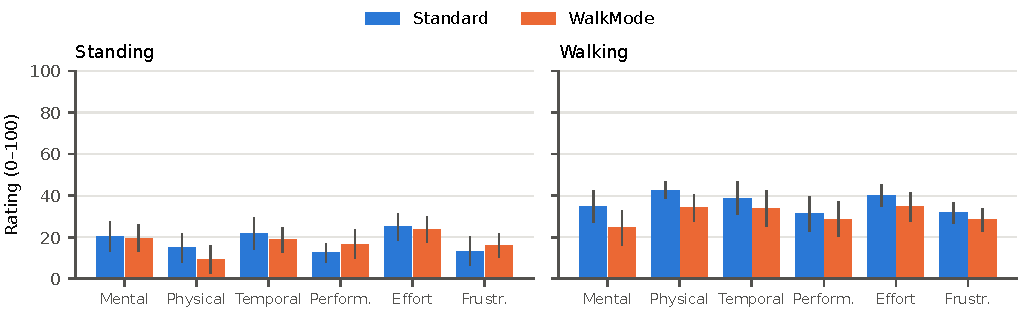
\includegraphics[width=\textwidth]{generated/fig_tlx.pdf}
\caption{NASA-TLX subscales (\DataSource). Error bars: 95\% CIs.}
\label{fig:tlx}
\end{figure*}

\subsection{Preference and comments (H5)}
While walking: \PrefWalking. While standing: \PrefStanding. Overall: \PrefOverall{} (Figure~\ref{fig:pref}). \todo{Likert medians from analysis/output/summary.md; two or three representative quotes from the open comments, grouped by theme.}

\begin{figure}[t]
\centering
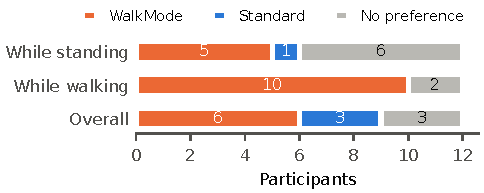
\includegraphics[width=\columnwidth]{generated/fig_pref.pdf}
\caption{Interface preference (\DataSource).}
\label{fig:pref}
\end{figure}

%% =====================================================================
\section{Discussion}
\todo{Rewrite once real results are in. Points worth addressing:}
\begin{itemize}
  \item \textbf{Adaptation where it matters.} Whether the benefit of larger targets appears only while walking (the Interface$\times$Mobility interaction) and whether stationary use is unaffected (H3). This pattern is the core argument for adapting the layout rather than enlarging it permanently.
  \item \textbf{Errors versus misses.} Wider gaps turn some near-misses that would have hit a neighbouring target into taps on empty space. A miss is cheaper to recover from than a wrong selection, especially in navigation, where a wrong selection opens the wrong page.
  \item \textbf{Cost of larger targets.} Fewer items fit on screen, so lists need more scrolling. Discuss the contacts-task times.
  \item \textbf{Detector behaviour.} Onset latency, false activations while standing, and whether participants noticed or minded the switch (Likert ``disruptive'' item). The touch-idle policy is a simple answer to moving targets.
\end{itemize}

\subsection{Limitations}
The sample is small and drawn from \todo{population}. Walking took place on a fixed indoor route at a self-selected pace, which differs from real streets with obstacles, traffic and divided attention. Participants knew which interface they were using, which can bias subjective ratings. The tasks were short selection tasks, and text entry and reading were not studied. The detector used fixed or briefly calibrated thresholds; walking speed was not controlled, and cadence served only as a proxy for pace. All participants used \todo{one device / their own devices}, so the physical size of a CSS pixel varies by device.

\subsection{Future work}
Natural next steps include continuous rather than binary adaptation (scaling sizes with motion intensity or gait), compensating for the systematic offsets of touches made while walking~\cite{goel2012walktype,music2016nomadic}, combining the layout change with reach-friendly placement of primary actions, and longer field deployments.

%% =====================================================================
\section{Conclusion}
\WM{} shows that a lightweight, browser-based walking detector and a simple, deferred change in target size and spacing can be deployed without special hardware. \todo{Conclude with the main empirical finding and its implication for mobile interface design.}

\begin{acks}
\todo{Course name and instructor; pilot participants.}
\end{acks}

\bibliographystyle{ACM-Reference-Format}
\bibliography{references}

\end{document}
